\chapter{ISR Inversion}
\label{chapter:inversion}
\thispagestyle{myheadings}

% set this to the location of the figures for this chapter. it may
% also want to be ../Figures/2_Body/ or something. make sure that
% it has a trailing directory separator (i.e., '/')!
\graphicspath{{5_Inversions/Figures/}}

%%%%%%%%%%%%%%%%%%%%%%%%%%%%%%%%%%%%%%%%%%%%%%%%%%%%%%%%%%%%%%%%%%%%%%%%%
This chapter will describe methods developed to invert the ISR space-time ambiguity function and improve on current reconstruction schemes. The first section will describe these inversion methods which are different types of constrained least squares. The next section will show examples using runs from STISRS to determine the utility of these inversion on reconstructing the true plasma parameters.

\section{Method Description}

As discussed in Section \ref{sec:imgrec}, the main trade-off between the two approaches is computational complexity versus accuracy of solution. Full profile analysis and other parametric regularization schemes require a large amount of computation to find a solution as the operator between the plasma parameters and ISR spectra is non-linear and thus various techniques from are not useful. With data-based regularization techniques the computational requirements are significantly lowered as on is performing a linear inversion. Still this can lead to estimated ACFs that can not be created by the incoherent scattering operator.

In order to reconstruct the field of plasma parameter values we treat the space-time ambiguity as a linear operator. This allows for the use of inversion schemes from image processing. In this case objective function will be 

\begin{equation}
\label{eqn:lstsqrs:opt}
\argmin\limits_{R} \| y_s(\tau_s,\mathbf{r}_s,t_s)- \int L(\tau_s,\mathbf{r}_s,t_s,\tau,\mathbf{r},t)R(\tau,\mathbf{r},t)dVdtd\tau \|^2.
\end{equation}

\noindent If Equation \ref{eqn:lstsqrs:opt} is discretized and the data and input lags are rasterized into a vector format it becomes 

\begin{equation}
\label{eqn:lstsqrs:disc}
\argmin\limits_{\mathbf{r}} \| \mathbf{y_s} -\mathbf{ L}\mathbf{r} \|^2.
\end{equation}





\section{Introduction}

Incoherent scatter radar (ISR) measures plasma parameters by fitting plasma parameters to an estimate of the auto correlation function (ACF) from the inherent fluctuations in electron density in the ionosphere. In order to perform this estimate the radar has to create an average of ACF over time and space. This averaging acts as a linear operator over time and space for the estimated ACFs and creates an ambiguity for the measurements. The direct impact of the operator on the measurement of plasma parameters can be difficult to assess as the relationship between plasma parameters and the ACF is non-linear. 

The development of the Advanced Modular Incoherent Scatter Radar (AMISR) systems, with its electronically-scannable antenna, have allowed for three dimensional reconstruction of plasma parameters. In order to analyze the performance of these systems the idea of the ambiguity function had to be extended to include the antenna beam pattern and the time dimension referred to as the space-time ambiguity function in  \cite{RDS:RDS20236}. 

With the linearity assumption many ideas in linear inverse theory can be applied. There is a large amount of literature in this area, mainly in image processing and reconstruction \cite{Karl:2005jy}, and could be used to invert the operator and improve the resolution of the measurement. 

This paper will cover the a method for inverting this space-time ambiguity function. In order to test this method we use synthetic data from the Simulation for ISR (SimISR), driven by a ionosphere plasma state parameters from a multi-fluid ionosphere model \cite{semeter:plasmatransport2012}. The following sections of this paper are as follows. Section \ref{sec:isramb} describes the ISR image formation process in the language of inverse theory. Following this, Section \ref{sec:isrlit} details the use of inverse theory in single dish ISR systems to reconstruct altitude profiles. Section \ref{sec:isralg} describes our specific algorithm that has been developed and following in Section \ref{sec:results}, we show results of these reconstructions.

%\section{ISR Space-Time Ambiguity}
%\label{sec:isramb}
%The ISR processing can be represented in the diagram seen in Figure \ref{fig:flow1}. The image formation process starts with a set of plasma parameters distributed in time and space. Each set of plasma parameters is then transformed to a set of ACFs using the operator represented by $g()$. The space time ambiguity function $L$ acts as a blurring operator one might see in a camera or numerous other types of sensors. The estimates are then fit and estimates of the plasma parameters, $\widehat{\boldsymbol{\theta}}$, are created. Often times these parameters are interpolated or projected back to the original Cartesian coordinate system, this is in a way applying the adjoint operator $L^*$ to the fitted plasma parameters to create a 
%
%\begin{figure}[!ht]
%\centering
%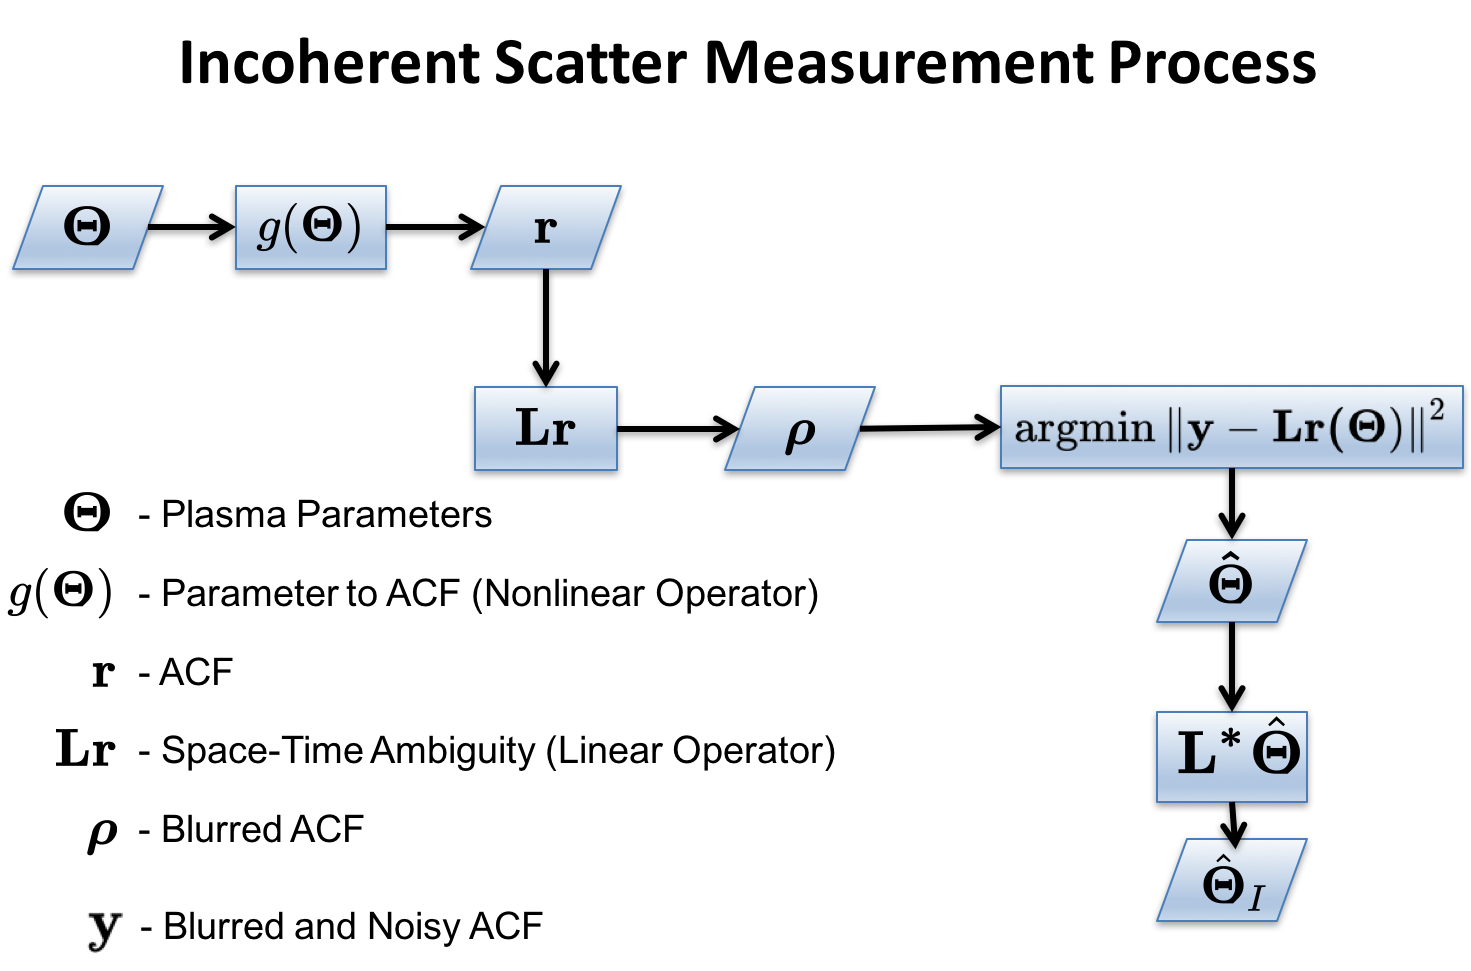
\includegraphics[width=.8\textwidth]{ladj}
%\caption{\label{fig:flow1}ISR image formation process.}
%\end{figure}
%
%The space-time ambiguity, $L(\tau_s,\mathbf{r}_s,t_s,\tau,\mathbf{r},t)$, can be treated as the kernel of a Fredholm integral equation of the first kind operating on the ACF, $R(\tau,\mathbf{r},t)$, which can change over space, $\mathbf{r}$, and time $t$, i.e.,
%
% \begin{equation}
%  \label{eqn:staf}
%  \rho(\tau_s,\mathbf{r}_s,t_s) =\int L(\tau_s,\mathbf{r}_s,t_s,\tau,\mathbf{r},t)R(\tau,\mathbf{r},t)dVdtd\tau,
%\end{equation}

%\noindent where the subscript $s$ represents the same variable but now discretely sampled by the radar. 
%
%The kernel is a separable function when the spatial coordinates are spherical, centered at the radar, where ($r,\theta,\phi)$ represent, range, azimuth and elevation respectively. This the changes Equation \ref{eqn:staf} as follows,
%
%\begin{equation}
%\label{eqn:stafbrok}
%\rho(\tau_s,\mathbf{r}_s,t_s)= \int G(t_s,t)F(\theta_s,\phi_s,\theta,\phi)W(\tau_s,r_s,\tau,r) R(\tau,\mathbf{r},t) dVdt d\tau,
%\end{equation}
%
%\noindent where $G(t_s,t)$ is the kernel for the time dimension, $F(\theta_s,\phi_s,\theta,\phi)$ is radar beam shape which acts as a kernel in azimuth and elevation, and $W(\tau_s,r_s,\tau,r) $ which is the range ambiguity function which acts as a kernel along range $r$ and lag $\tau$. The derivation of this operator can be seen in \cite{RDS:RDS20236}.
%
%
%\begin{figure}[!ht]
%    \centering
%    \begin{subfigure}[b]{0.47\textwidth}
%        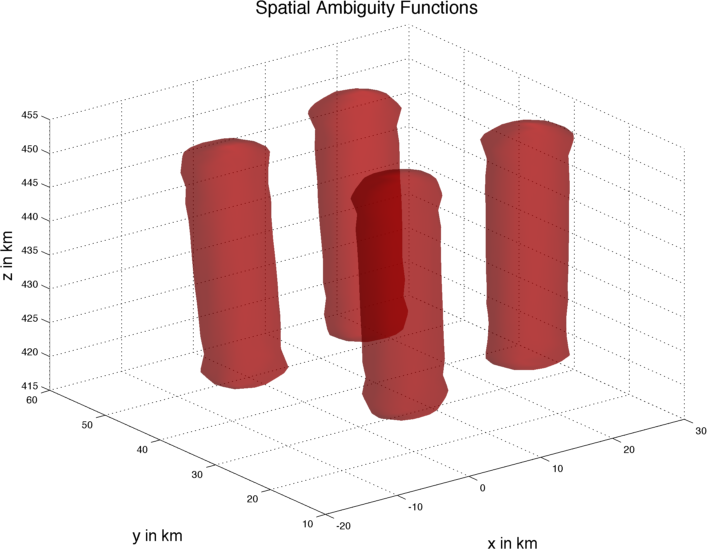
\includegraphics[width=\textwidth]{spaceamb}
%        \caption{Stationary.}
%        \label{fig:Amb1}
%    \end{subfigure}
%    ~ %add desired spacing between images, e. g. ~, \quad, \qquad, \hfill etc. 
%      %(or a blank line to force the subfigure onto a new line)
%    \begin{subfigure}[b]{0.47\textwidth}
%        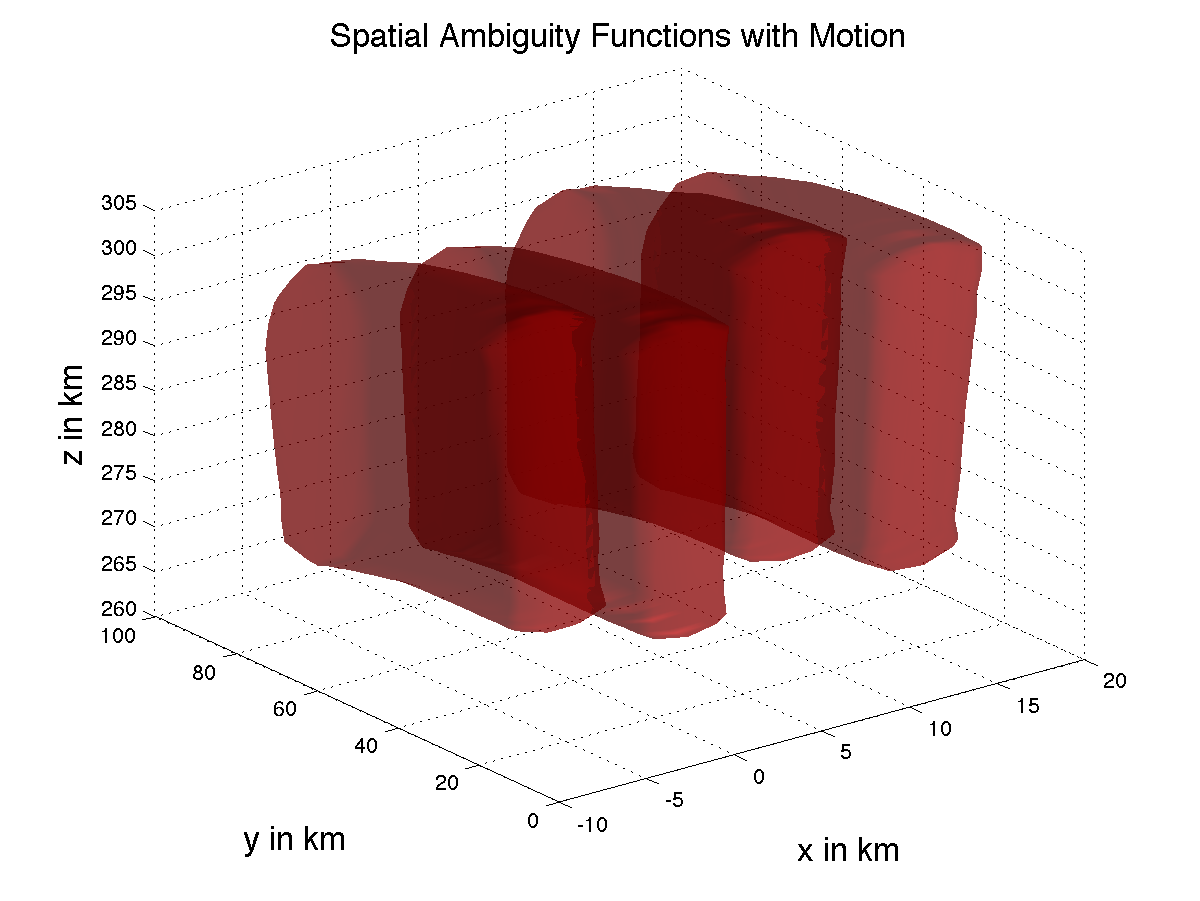
\includegraphics[width=\textwidth]{spaceambmoving}
%        \caption{With 500 m/s drift.}
%        \label{fig:Ambmoving}
%    \end{subfigure}
%
%    \caption{Space time ambiguity function.}\label{fig:Ambboth}
%\end{figure}
%
%The ambiguity found in Cartesian space in Figure \ref{fig:Amb1}. The ambiguity is interesting in a number of ways. First it is non-isotropic in space so it is important to know the orientation of the beam and its shape otherwise this may cause errors in any inversion scheme. Another aspect is that the blurring in incurs is shift variant in space, so it is not a convolution and thus any methods specific for those problems will not apply. Lastly, like in cameras if there is motion in the plasma during the integration period then a motion blur will also be added. This will change the ambiguity in the rest frame of the plasma to be closer to what is seen in Figure \ref{fig:Ambmoving}.

%In order to estimate the ACFs a large number of pulses need to be integrated. Using the central limit theorem on can argue that the estimated ACFs become Normally distributed random variable \cite{papoulis2002}. The radar data can be modeled as follows $ y_s\sim \mathcal{CN}(\rho,\mathbf{C})$, where $\mathbf{C}$ is the covariance matrix of the ACFs, or even,
%
%\begin{equation}
%\label{eqn:procsignal}
% y_s(\tau_s,\mathbf{r}_s,t_s) = \rho(\tau_s,\mathbf{r}_s,t_s) + w(\tau_s,\mathbf{r}_s,t_s),
%\end{equation}
%
%\noindent where $w(\tau_s,\mathbf{r}_s,t_s)$ is the ACF of the noise process. 
%
%For standard ISR processing, the plasma parameters at each point in space and time individually. The cost function used is tries to reduce the error between the model ACF and the measured value in the least squares sense,
%
%\begin{equation}
%\label{eqn:lstsqrs}
%\widehat{\boldsymbol{\theta}_s} = \argmin\limits_{\boldsymbol{\theta}} \|y_s - g(\boldsymbol{\theta}_s) \|^2.
%\end{equation}
%
%\noindent The Levenberg-Marquart algorithm is often used to fit the plasma parameters to the final estimate ACFs \cite{levenberg1944,marquardt:1963,nikoukar2008}.
%%%%%%%%%%%%%%%%%%%%%%%%%%%%%%%%%%%%%%%%%%%%%%%%%%%%%%%%%%%%%%%%%%%%%%%
\section{Inversion Schemes}
\label{sec:isrlit}
The ambiguity function across range has been well studied and there have been a number of different methods proposed to reduce its impact on ISR measurements,
\cite{RDS:RDS3308,hysell2008,nikoukar2008,Virtanen:20082vx}. These methods come down to two different types of regularization. The first type Full Profile Analysis which is detailed in \cite{RDS:RDS3308} and \cite{hysell2008}, inverts the entire ISR process, even the non-linear step when moving between the parameter space and ACF space. This allows for parametric regularization which can include known physical constraints. The second type inverts only the range ambiguity as a linear operator and regularizes the estimated ACF. This is detailed in \cite{nikoukar2008} and\cite{Virtanen:20082vx}, and will be referred to data-based regularization.

The main trade-off between the two approaches is computational complexity versus accuracy of solution. Full profile analysis and other parametric regularization schemes require a large amount of computation to find a solution as the operator between the plasma parameters and ISR spectra is non-linear and thus various techniques from are not useful. With data-based regularization techniques the computational requirements are significantly lowered as on is performing a linear inversion. Still this can lead to estimated ACFS that can not be created by the incoherent scattering operator.


The best way to compare and contrast the two formats is to first pose the problem in a vector format, first each point in lag, length $N_l$, time, length $N_t$ and space, length $N_s$, are vectorized along the index $i$. This will create a $N_lN_sN_t\times 1$ length vector 

\begin{equation}
\label{eqn:vec1}
\mathbf{y}=[y(\tau_0,\mathbf{r}_0,t_0), y(\tau_1,\mathbf{r}_1,t_1),..., y(\tau_{N_l N_s N_t -1}, \mathbf{r}_{N_l N_s N_t -1}, t_{N_l N_s N_t -1})]^T.
\end{equation}

The next step will be to discretize the input space which will be represented by the vector $\mathbf{x}$. Like $\mathbf{y}$ each point in lag, length $N_v$, time, length $N_p$ and space, length $N_c$, are vectorized along the index $j$. The resulting $N_vN_pN_c\times 1$ length vector is the following,

\begin{equation}
\label{eqn:vecr}
\mathbf{x}=[x(\tau_0,\mathbf{r}_0,t_0), y(\tau_1,\mathbf{x}_1,t_1),..., y(\tau_{N_c N_p N_c -1}, \mathbf{x}_{N_v N_p N_c -1}, t_{N_v N_p N_c -1})]^T.
\end{equation}

The space-time ambiguity can be represented in a fully discretized form as the matrix $\mathbf{L}$. Substituting this into Equation \ref{eqn:procsignal} it becomes,

\begin{equation}
\label{eqn:procsignalvec}
 \mathbf{y} = \mathbf{L}\mathbf{x}+ \mathbf{w},
\end{equation}
\noindent where $\mathbf{x}$ is the intrinsic ACF in the Cartesian Coordinate space, and $\mathbf{w}$ is the vector of the noise process.

For the case of parametric based reconstruction schemes such as full profile analysis try to reconstruct the full set of plasma parameters at each point in time and space, represented as the matrix $\boldsymbol{\Theta}$. The cost function for this is the following, 

\begin{equation}
\label{eqn:lstsqrsvecpb}
\widehat{\boldsymbol{\Theta}} = \argmin\limits_{\boldsymbol{\Theta}} \|\mathbf{y} -\mathbf{L}\mathbf{ g}(\boldsymbol{\Theta}) \|^2 + \boldsymbol{\alpha}\cdotp\mathbf{f}(\boldsymbol{\Theta}),
\end{equation}

\noindent where $\mathbf{f}(\boldsymbol{\Theta})$ is a vector of constraints functionals based on the plasma parameters, $\boldsymbol{\alpha}$ is a vector that holds the different weightings for these constraints.

With the data based reconstruction the inversion is based on removing the affect of the space time ambiguity function and then fitting the plasma parameters after. The cost function, similar to Equation \ref{eqn:lstsqrsvecpb} is the following

\begin{equation}
\label{eqn:lstsqrsvecdb}
\widehat{\mathbf{x}} = \argmin\limits_{\mathbf{x}} \|\mathbf{y} -\mathbf{Lx} \|^2 + \boldsymbol{\gamma}\cdotp\mathbf{f}(\mathbf{x}),
\end{equation}

\noindent where $\mathbf{f}(\mathbf{x})$ is a vector of constraint functionals based on the ACFs, $\boldsymbol{\gamma}$ is a vector that holds the different weightings for these constraints. The ACFs are then fit to plasma parameters at one point in space and time as in Equation \ref{eqn:lstsqrs}.

%The best way to compare and contrast the two formats is to first pose the problem in a vector format, first each time and spatial vector are rasterized along the index $i$. Next the discrete estimate of each ACF can be placed in an $L$ length single vector for each space-time index $i$,
%
%\begin{equation}
%\label{eqn:vec1}
%\mathbf{y}_i=[y(\tau_0,\mathbf{r}_i,t_i), y(\tau_1,\mathbf{r}_i,t_i),..., y(\tau_{L-1},\mathbf{r}_i,t_i)].
%\end{equation}
%
%\noindent This vector $y_i$ can be come the $i^{th}$ row in the matrix $\mathbf{Y}$,
%
%\begin{equation}
%\label{eqn:matall}
%\mathbf{Y}=[\mathbf{y}_0^T,\mathbf{y}_1^T, ..., \mathbf{y}_{NM}^T]^T
%\end{equation}
%
%\noindent where $N$ is number of locations that were sampled by the radar and $M$ is the number of times. With this representation Equation \ref{eqn:procsignal} becomes
%
%\begin{equation}
%\label{eqn:matsigproc}
%\mathbf{Y} = \boldsymbol{\rho} + \mathbf{W},
%\end{equation}
%
%\noindent where $\mathbf{W}$ is the $NM\times L$ noise matrix. 




%There may be some way in between. In \cite{Oktem:2014ju} data from spectral imagers are inverted with a nonlinear step involved. This type of technique only takes into account data from pixels that are near to the point of interest. This could be useful in ISR due to the fact that contributions from far away points is rather small due to the beam pattern. 
%
%Another aspect that needs to be explored is the possibility of using an iterative technique that where the ACFs are estimated and then fit to plasma parameters iteratively. This could yield a solution that would reduce computational complexity but improve the accuracy of the solutions.

\section{Inversion Method}
\label{sec:isralg}
Due to the size of the problem the inversion methods focused on here will be a data based regularization cost functions of the type seen Equation \ref{eqn:lstsqrsvecdb}. The space time ambiguity matrix $\mathbf{L}$ has a block matrix form with the sub-matrix $\mathbf{K}$ representing the spatial ambiguity. This block structure can be seen in Equation \ref{eqn:kmat},

\begin{equation}
\label{eqn:kmat}
\mathbf{L}= \begin{bmatrix}\mathbf{K}&\cdots&\mathbf{K}&\mathbf{0}&\cdots&&\mathbf{0}\\
\mathbf{0}&\cdots&&\mathbf{K}&\cdots&\mathbf{K}&\mathbf{0}\\
\vdots&&&\ddots&&&\vdots\\
\mathbf{0}&&&\cdots&\mathbf{K}&\cdots&\mathbf{K}
\end{bmatrix},
\end{equation}

\noindent where $\mathbf{0}$ is a matrix of zeros the same size as $\mathbf{K}$. This representation has some advantages as instead of inverting the whole matrix different blocks can be inverted at a time. This still leads to rather large matrices to invert because the number of rows grow with the number of number of times integrated. 

Another representation that can drop the calculations down further entails adjusting the spatial ambiguity to take into account the velocity of the plasma. Using a Galilean Transform like in \cite{RDS:RDS20236}, the set of $\mathbf{K}$ matrices for each time integration can become a single matrix $\mathbf{A}_{m,n}$. This form is shown as the following:

\begin{equation}
\label{eqn:amat}
\mathbf{L}= \begin{bmatrix}
\mathbf{A}_{0,0}&\mathbf{0}&\cdots&\mathbf{0}\\
 \mathbf{0}&\mathbf{A}_{1,1}&\mathbf{0}&\\
 \vdots&&\ddots&\vdots\\
 \mathbf{0}&\cdots&&\mathbf{A}_{N_T-1,N_T-1}
\end{bmatrix}.
\end{equation}

\noindent Each individual matrix can then be inverted. This will now reconstruct the ACFs in the moving frame of reference. This then assumes a stationary morphology of the plasma parameters. 

To invert the ACFs we invert each individual time frame and lag of the ACF separately. It creates the following cost function

\begin{equation}
\label{eqn:lstsqrsvecdblag}
\widehat{\mathbf{x}_{m,l}} = \argmin\limits_{\mathbf{x}_{m,l}} \|\mathbf{y}_{m,l} -\mathbf{L}_{m,l}\mathbf{x}_{m,l} \|^2 + \boldsymbol{\gamma}\cdotp\mathbf{f}(\mathbf{x}_{m,l}),
\end{equation}
\noindent where the indexes $m$ and $l$ represent time and lag respectively. In order to solve the cost functions the package CVXPY is used \cite{cvxpy}.

For this paper the specific cost functions will be used. The first will be an constraint on the $l^2$-norm of the solution $\mathbf{x}_{m,l}$, which can represented as the following cost function,
\begin{equation}
\label{eqn:tikpow}
\widehat{\mathbf{x}_{m,l}} = \argmin\limits_{\mathbf{x}_{m,l}} \|\mathbf{y}_{m,l} -\mathbf{L}_{m,l}\mathbf{x}_{m,l} \|^2 +\gamma_{m,l} \|\mathbf{x}_{m,l}\|^2.
\end{equation}

\noindent This type of regularization is generally referred to as Tikhonov Regularization \cite{Karl:2005jy}.

The next type of constraint will also be $l^2$-norm constraint on the solution, Tikhonov Regularization, except that it will be on $\mathbf{D}\mathbf{x}_{m,l}$, a numerical approximation to the spatial gradient of $\mathbf{x}_{m,l}$. The cost function is the following,

\begin{equation}
\label{eqn:tikD}
\widehat{\mathbf{x}_{m,l}} = \argmin\limits_{\mathbf{x}_{m,l}} \|\mathbf{y}_{m,l} -\mathbf{L}_{m,l}\mathbf{x}_{m,l} \|^2 + \gamma_{m,l} \|\mathbf{D}\mathbf{x}_{m,l}\|^2.
\end{equation}

\noindent The last constraint similar to the that in Equation \ref{eqn:tikpow} but instead using an $l^1$-norm,
\begin{equation}
\label{eqn:tv}
\widehat{\mathbf{x}_{m,l}} = \argmin\limits_{\mathbf{x}_{m,l}} \|\mathbf{y}_{m,l} -\mathbf{L}_{m,l}\mathbf{x}_{m,l} \|^2 + \gamma_{m,l} \|\mathbf{D}\mathbf{x}_{m,l}\|.
\end{equation} 

\noindent This constraint is generally referred to \textit{total variations} and has been used in image processing \cite{Rudin:1992kn}

\section{Results}
\label{sec:results}
In order to test the the results of the inversion method a set of plasma parameters is used from \cite{Perry:2015jf} which show an auroral arc moving through the field of view at 200 m/s. The background plasma parameter values can be seen in Figure \ref{fig:plparamst0inv}. The field align current (FAC), which drives the arc, creates enhancements in electron density, electron and ion temperature. Also of importance is the plasma cavity which is co-located with the ion temperature enhancement and slightly ahead of the electron density enhancement. The specific features can be seen in Figure \ref{fig:plparamst960inv} and the same parameters 45 seconds later as the arc travels through the field of view in Figure \ref{fig:plparamst1005inv}

\begin{figure}[!ht]
\centering
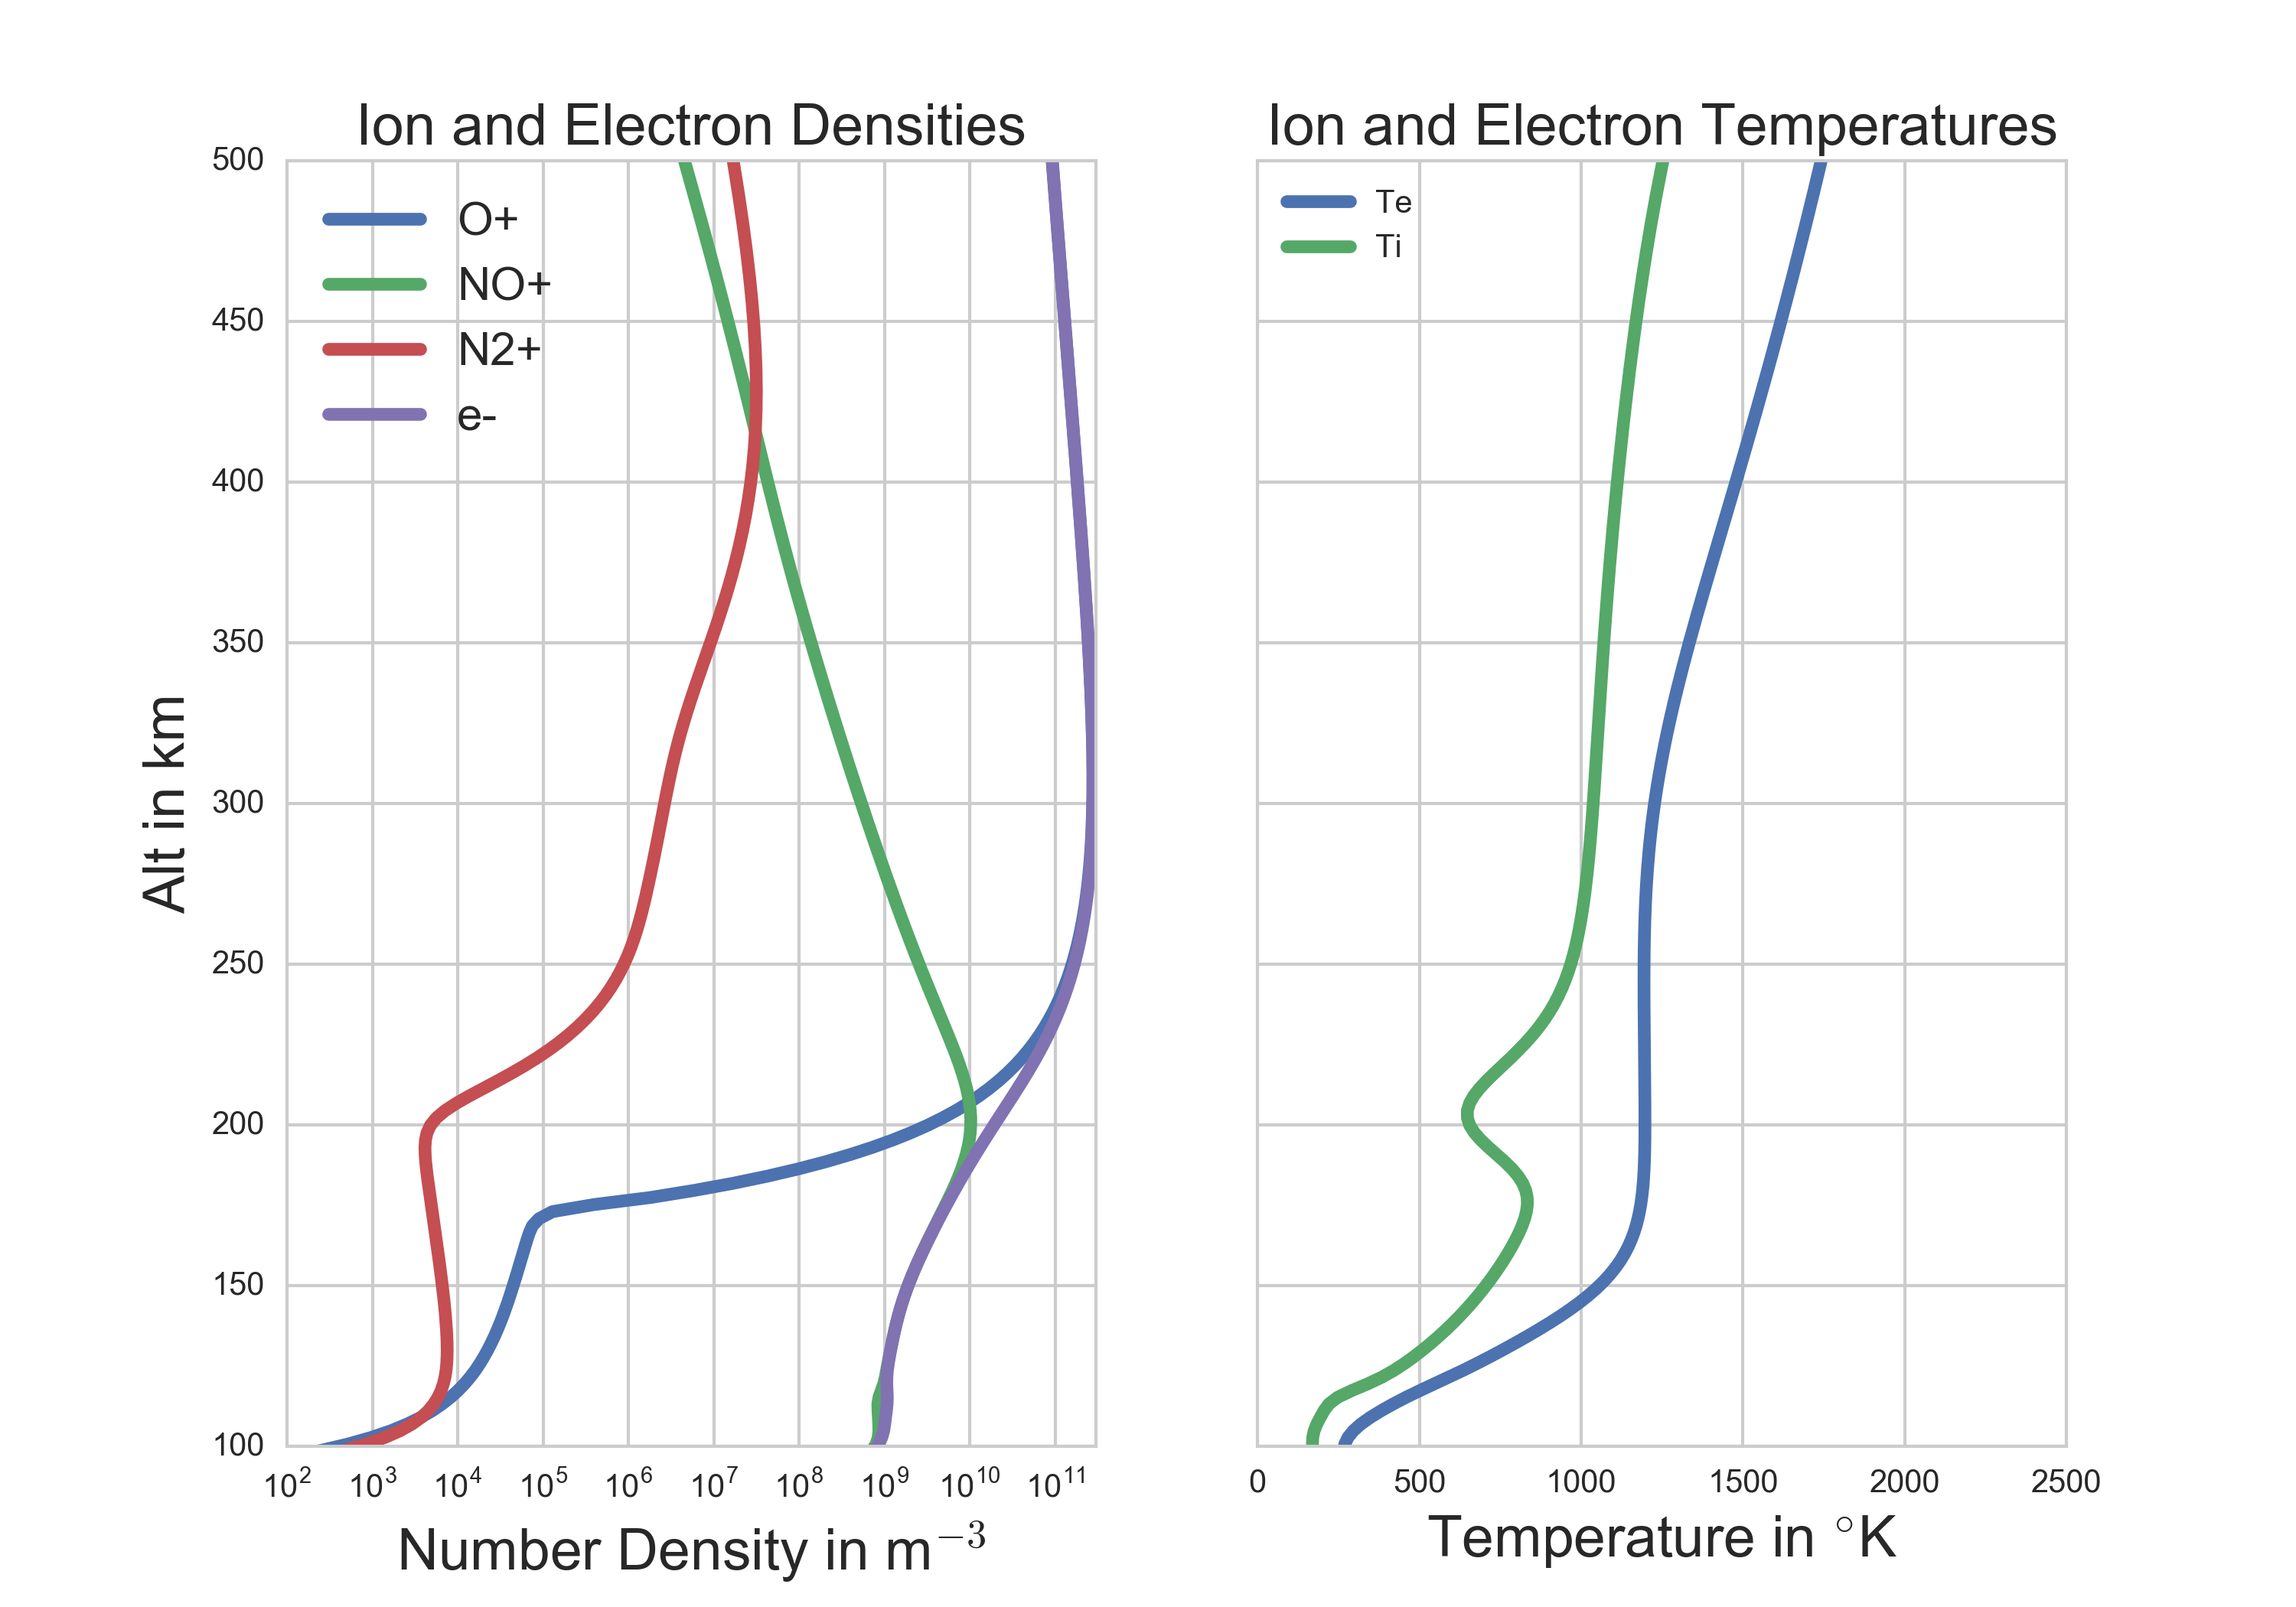
\includegraphics[width=4in]{backgroundallparams}
\caption{Background ionospheric parameters ($N_e$, $T_e$, $T_i$) along with number density of ion species, used for simulations.}
\label{fig:plparamst0inv}
\end{figure}

\begin{figure}[!ht]
\centering
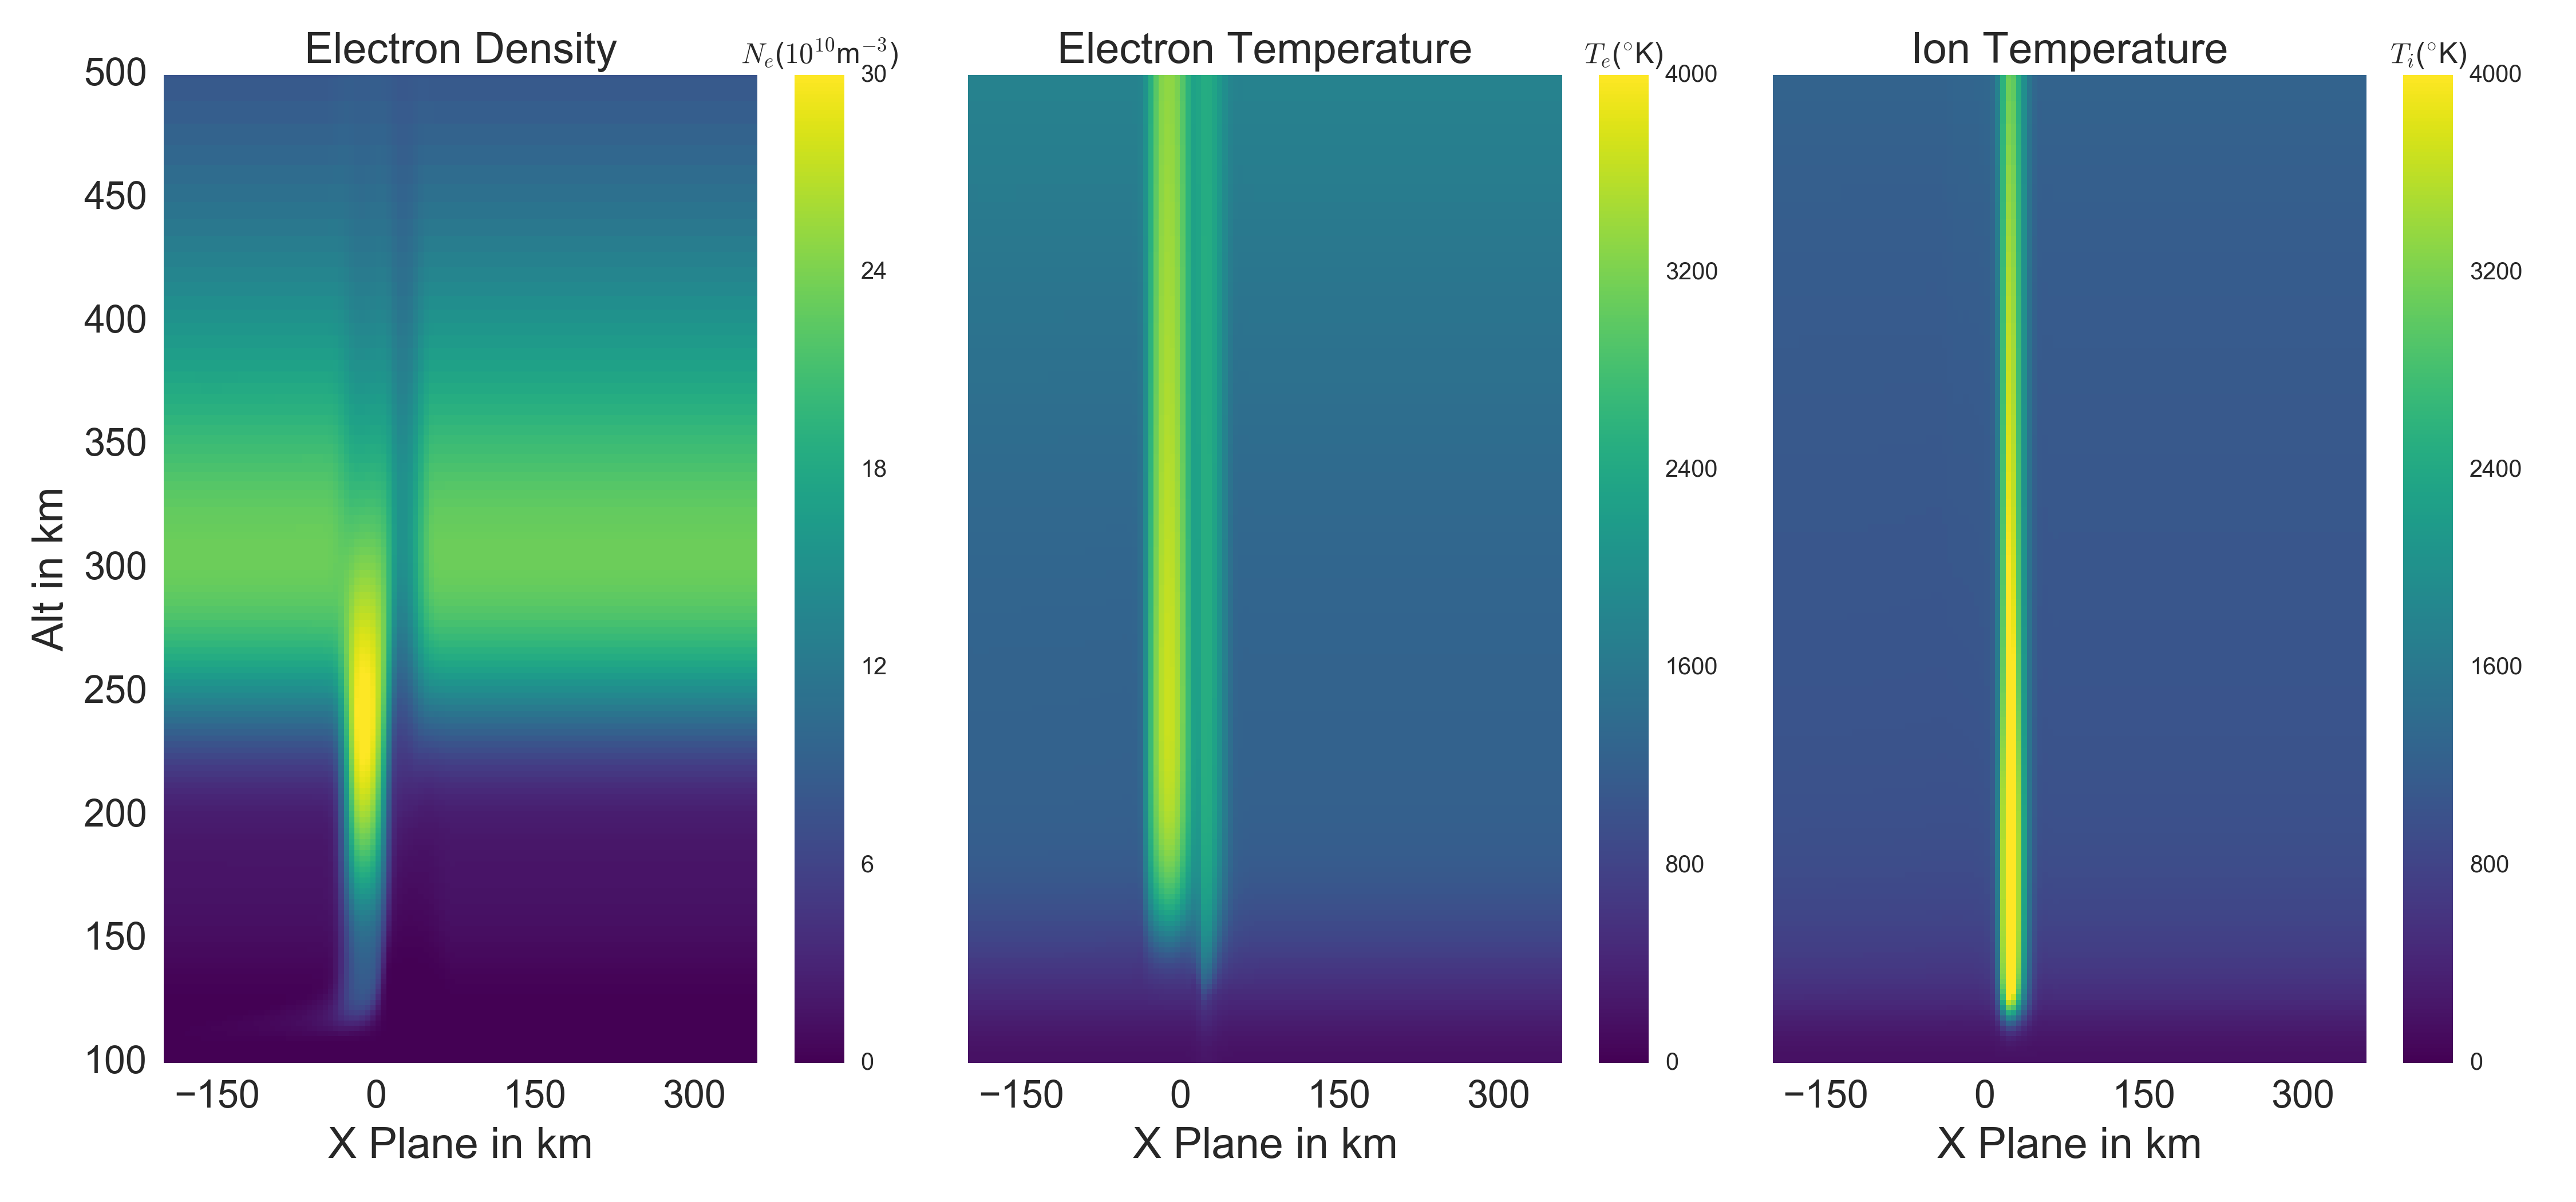
\includegraphics[width=6in]{0960_15_int}
\caption{Perturbations to Figure \ref{fig:plparamst0} due to an imposed current system of .875 $\mu$A/m$^2$ at $t=960$ s, auroral arc.}
\label{fig:plparamst960inv}
\end{figure}


\begin{figure}[!ht]
\centering
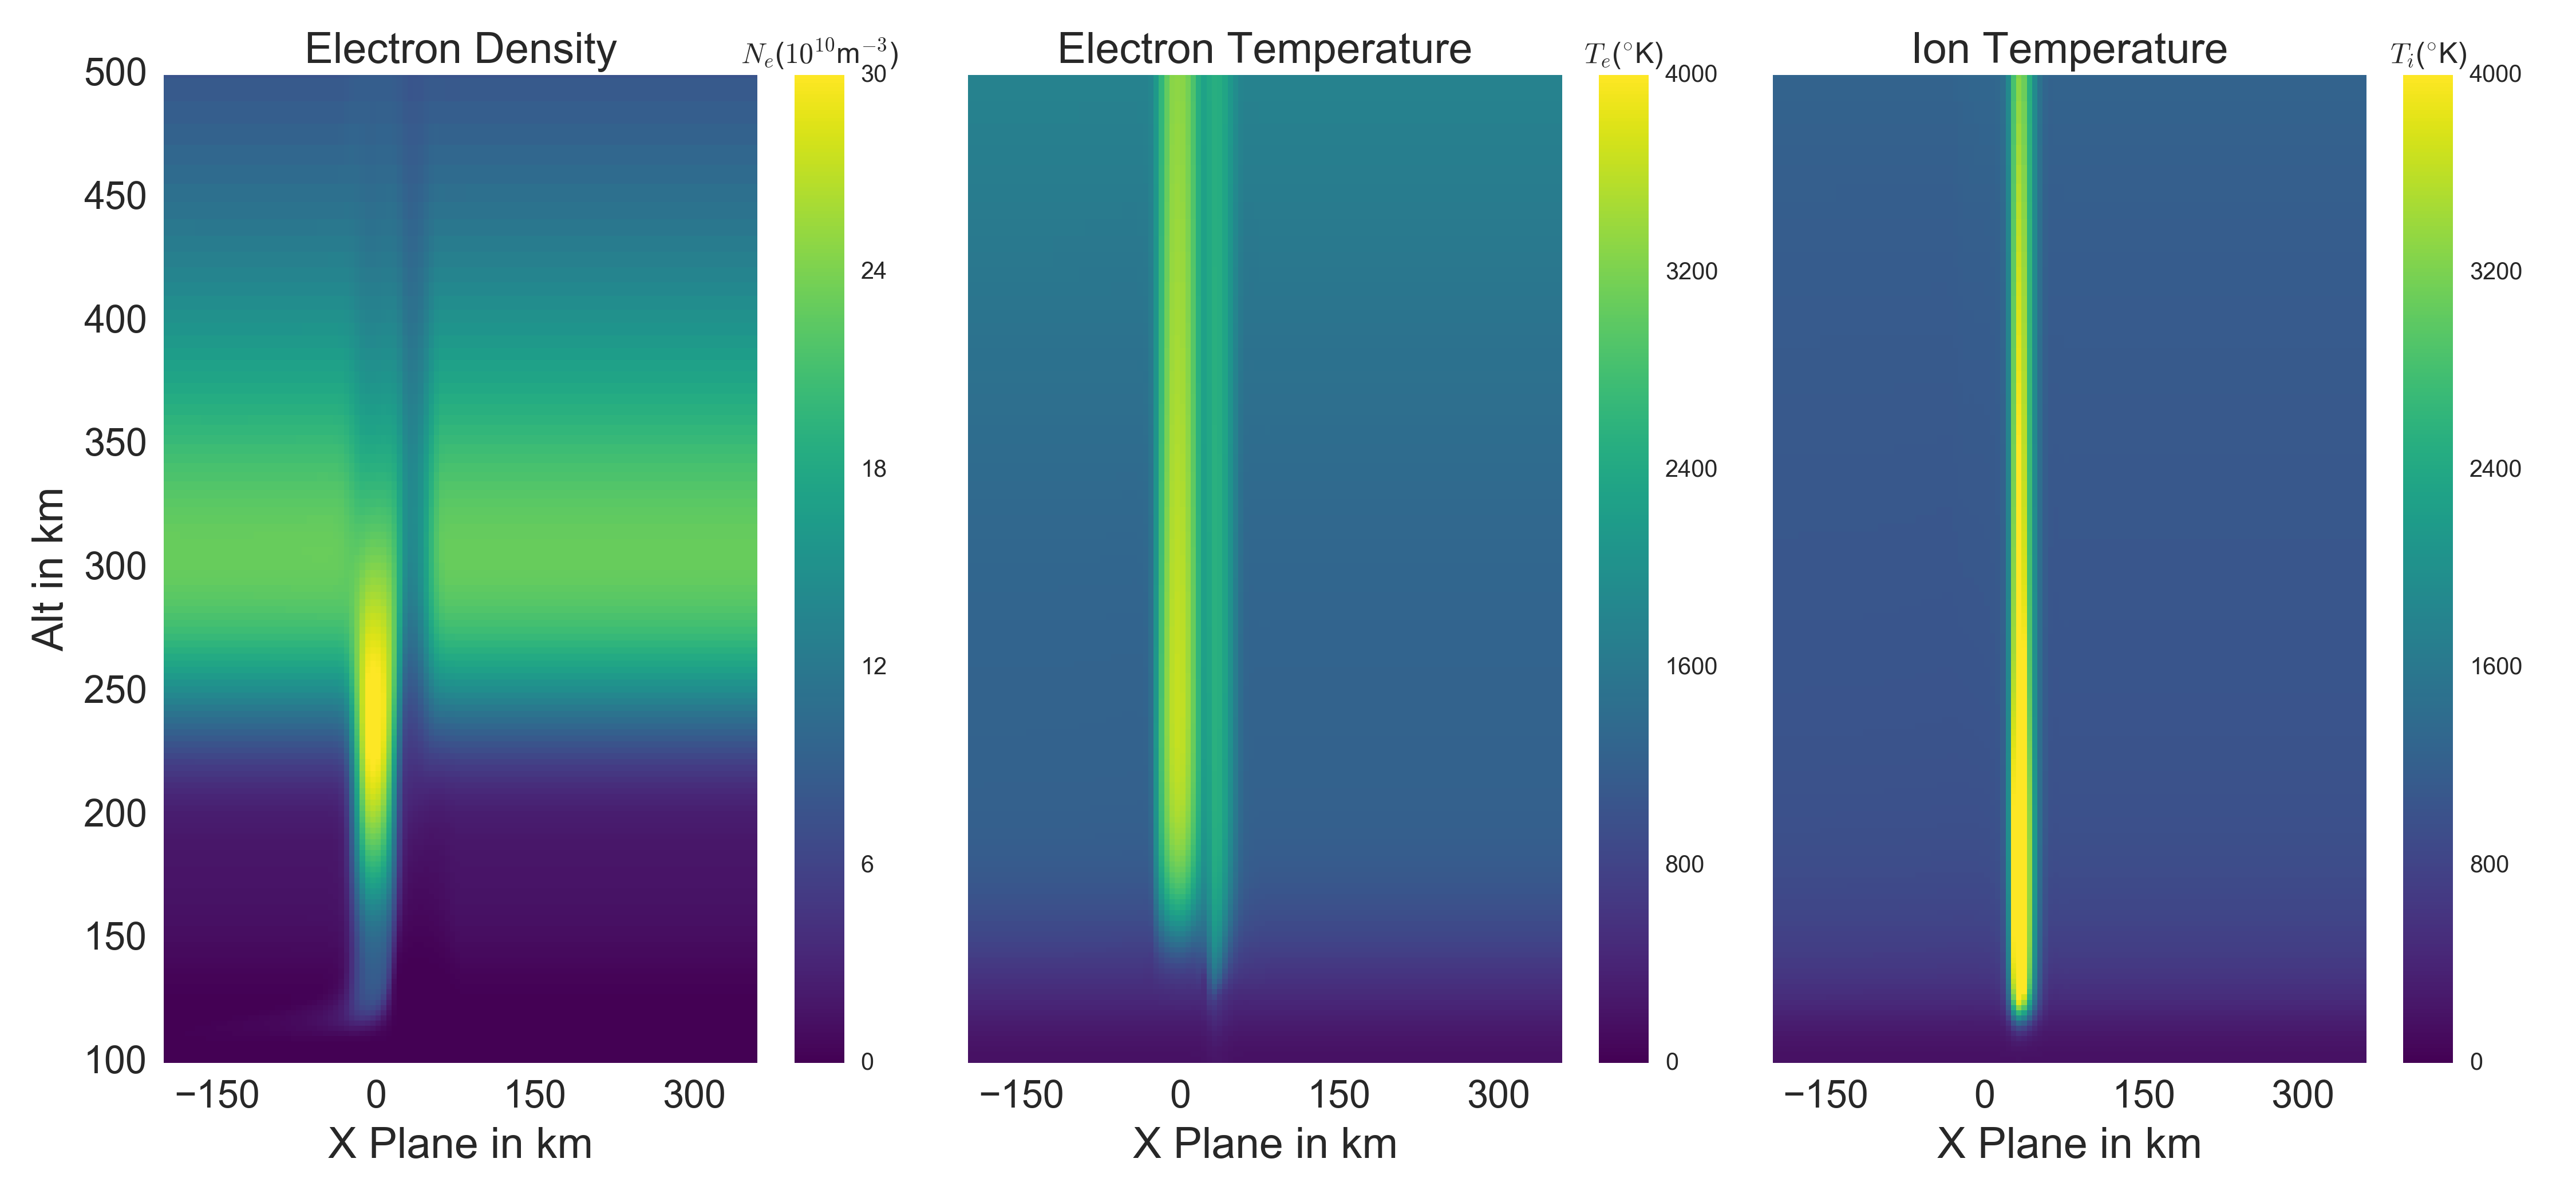
\includegraphics[width=6in]{1005_15_int}
\caption{Perturbations to Figure \ref{fig:plparamst0} due to an imposed current system of .875 $\mu$A/m$^2$ at $t=1005$ s, auroral arc.}
\label{fig:plparamst1005inv}
\end{figure}

The results using standard fitting and then linear interpolating the results, can be seen in Figure \ref{fig:fplparamst60inv} and the associated errors in Figure \ref{fig:fplparamst60errinv}. The enhancements in $T_i$ and $T_e$ are visible although noisy. Also the depletion in $N_e$ is visible although this can be tied to the geometry of the beam pattern. The values seen in these patterns are also much larger then most of the errors seen in Figure \ref{fig:fplparamst60errinv} so there is some confidence in these fits.

% fitted data no inversion
\begin{figure}[!ht]
\centering
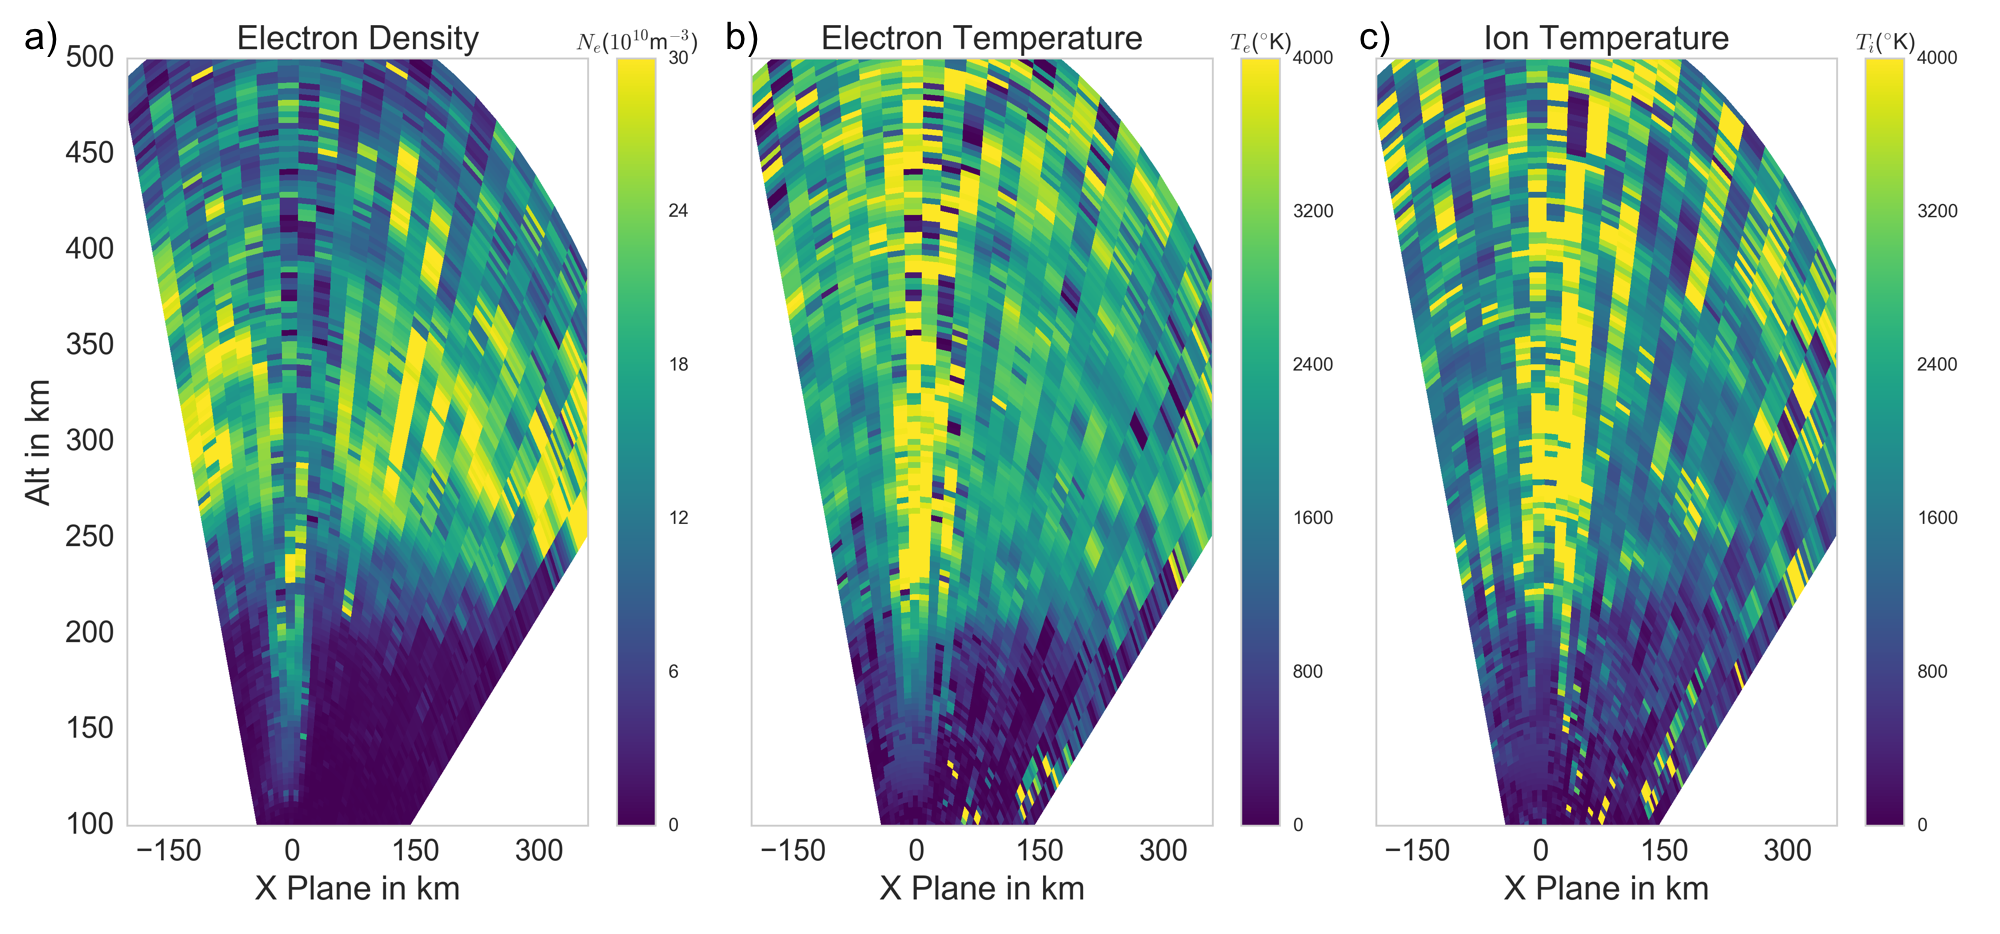
\includegraphics[width=6in]{0960_60_int}
\caption{Fitted Plasma Parameters at $t=960$ s with 60 second integration.}
\label{fig:fplparamst60inv}
\end{figure}

\begin{figure}[!ht]
\centering
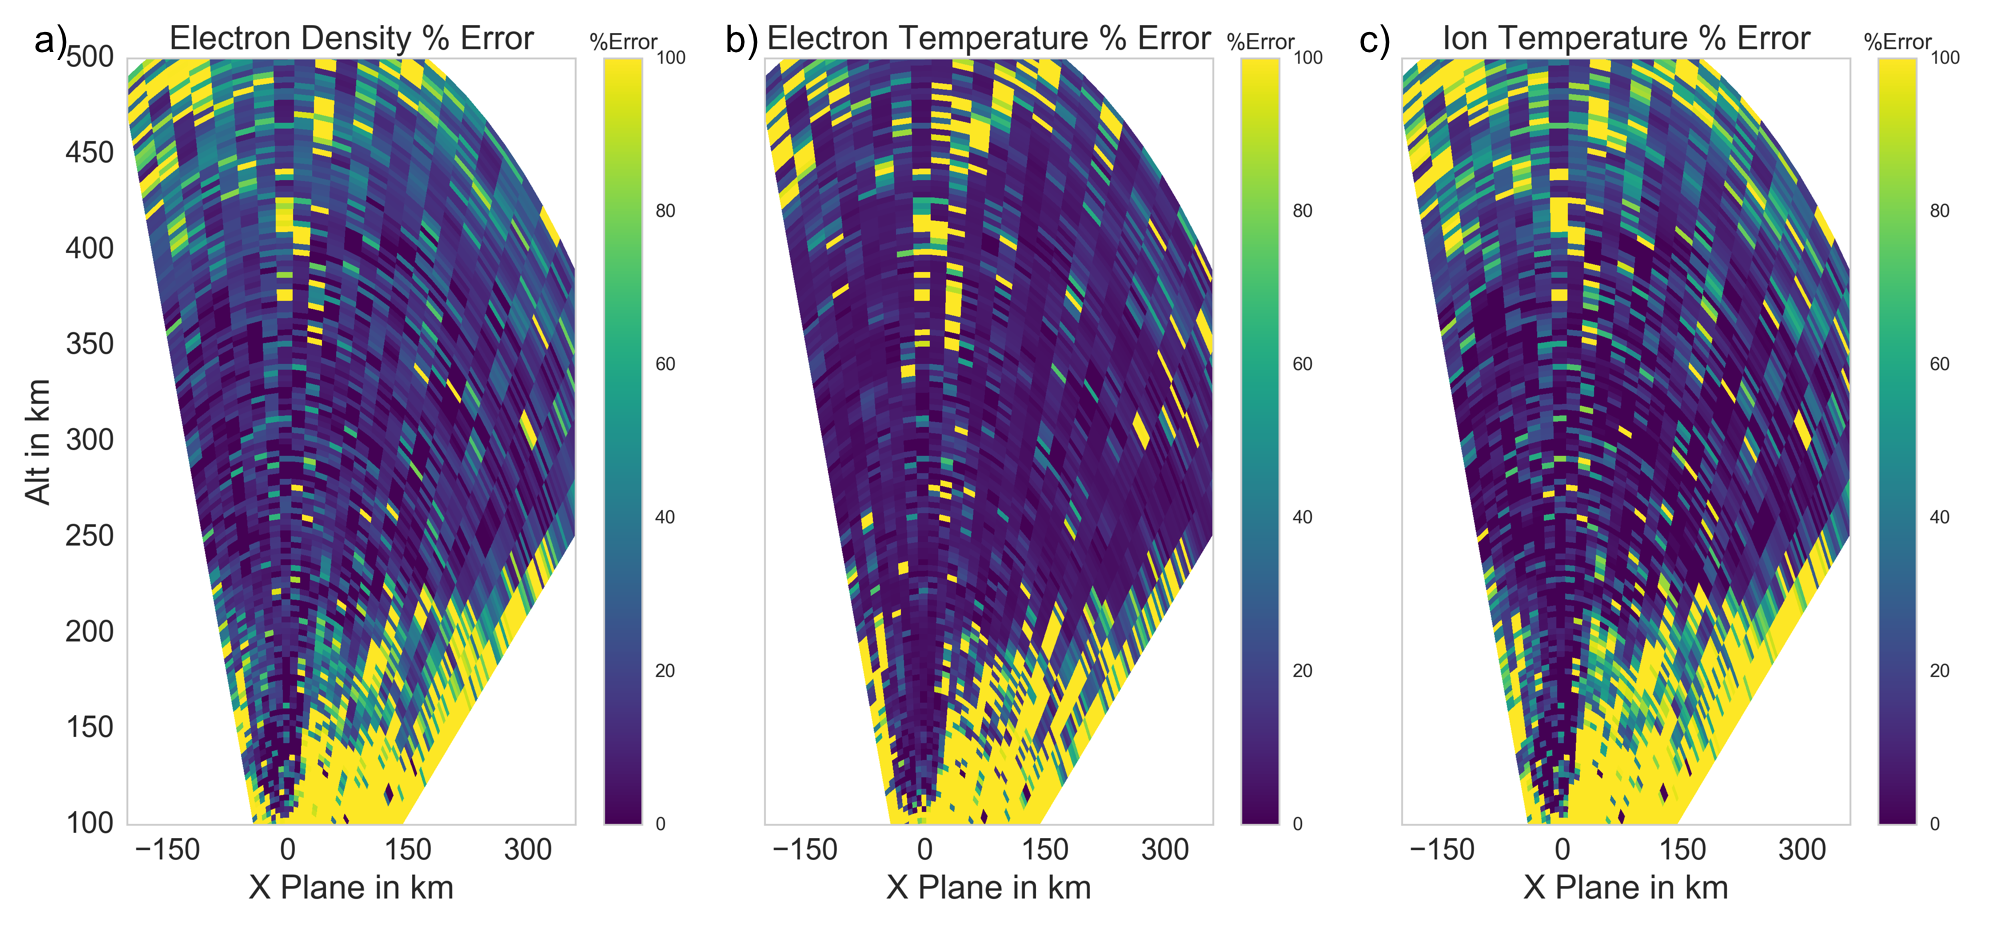
\includegraphics[width=6in]{0960_60_int_err}
\caption{Estimated errors from fitted Plasma Parameters at $t=960$ s with 60 second integration.}
\label{fig:fplparamst60errinv}
\end{figure}

% inverted and fitted data
The results of using the inversion algorithms can be seen in Figures \ref{fig:tikpow}, \ref{fig:tikD} and \ref{fig:tv}. In order to find the right values for the $\gamma$ term for each type of inversion the algorithm is run and the value that retrieves the lowest mean squared error between the inverted lag and the origin input is used. 

The case using using Tikhonov regularization where the $l^2$-norm of $\mathbf{x}_{m,l}$ is constrained is shown in Figure \ref{fig:tikpow}. This specific case shows an inability of the constraint to fill in data that may be lost due to the specific beam position. 

\begin{figure}[!ht]
\centering
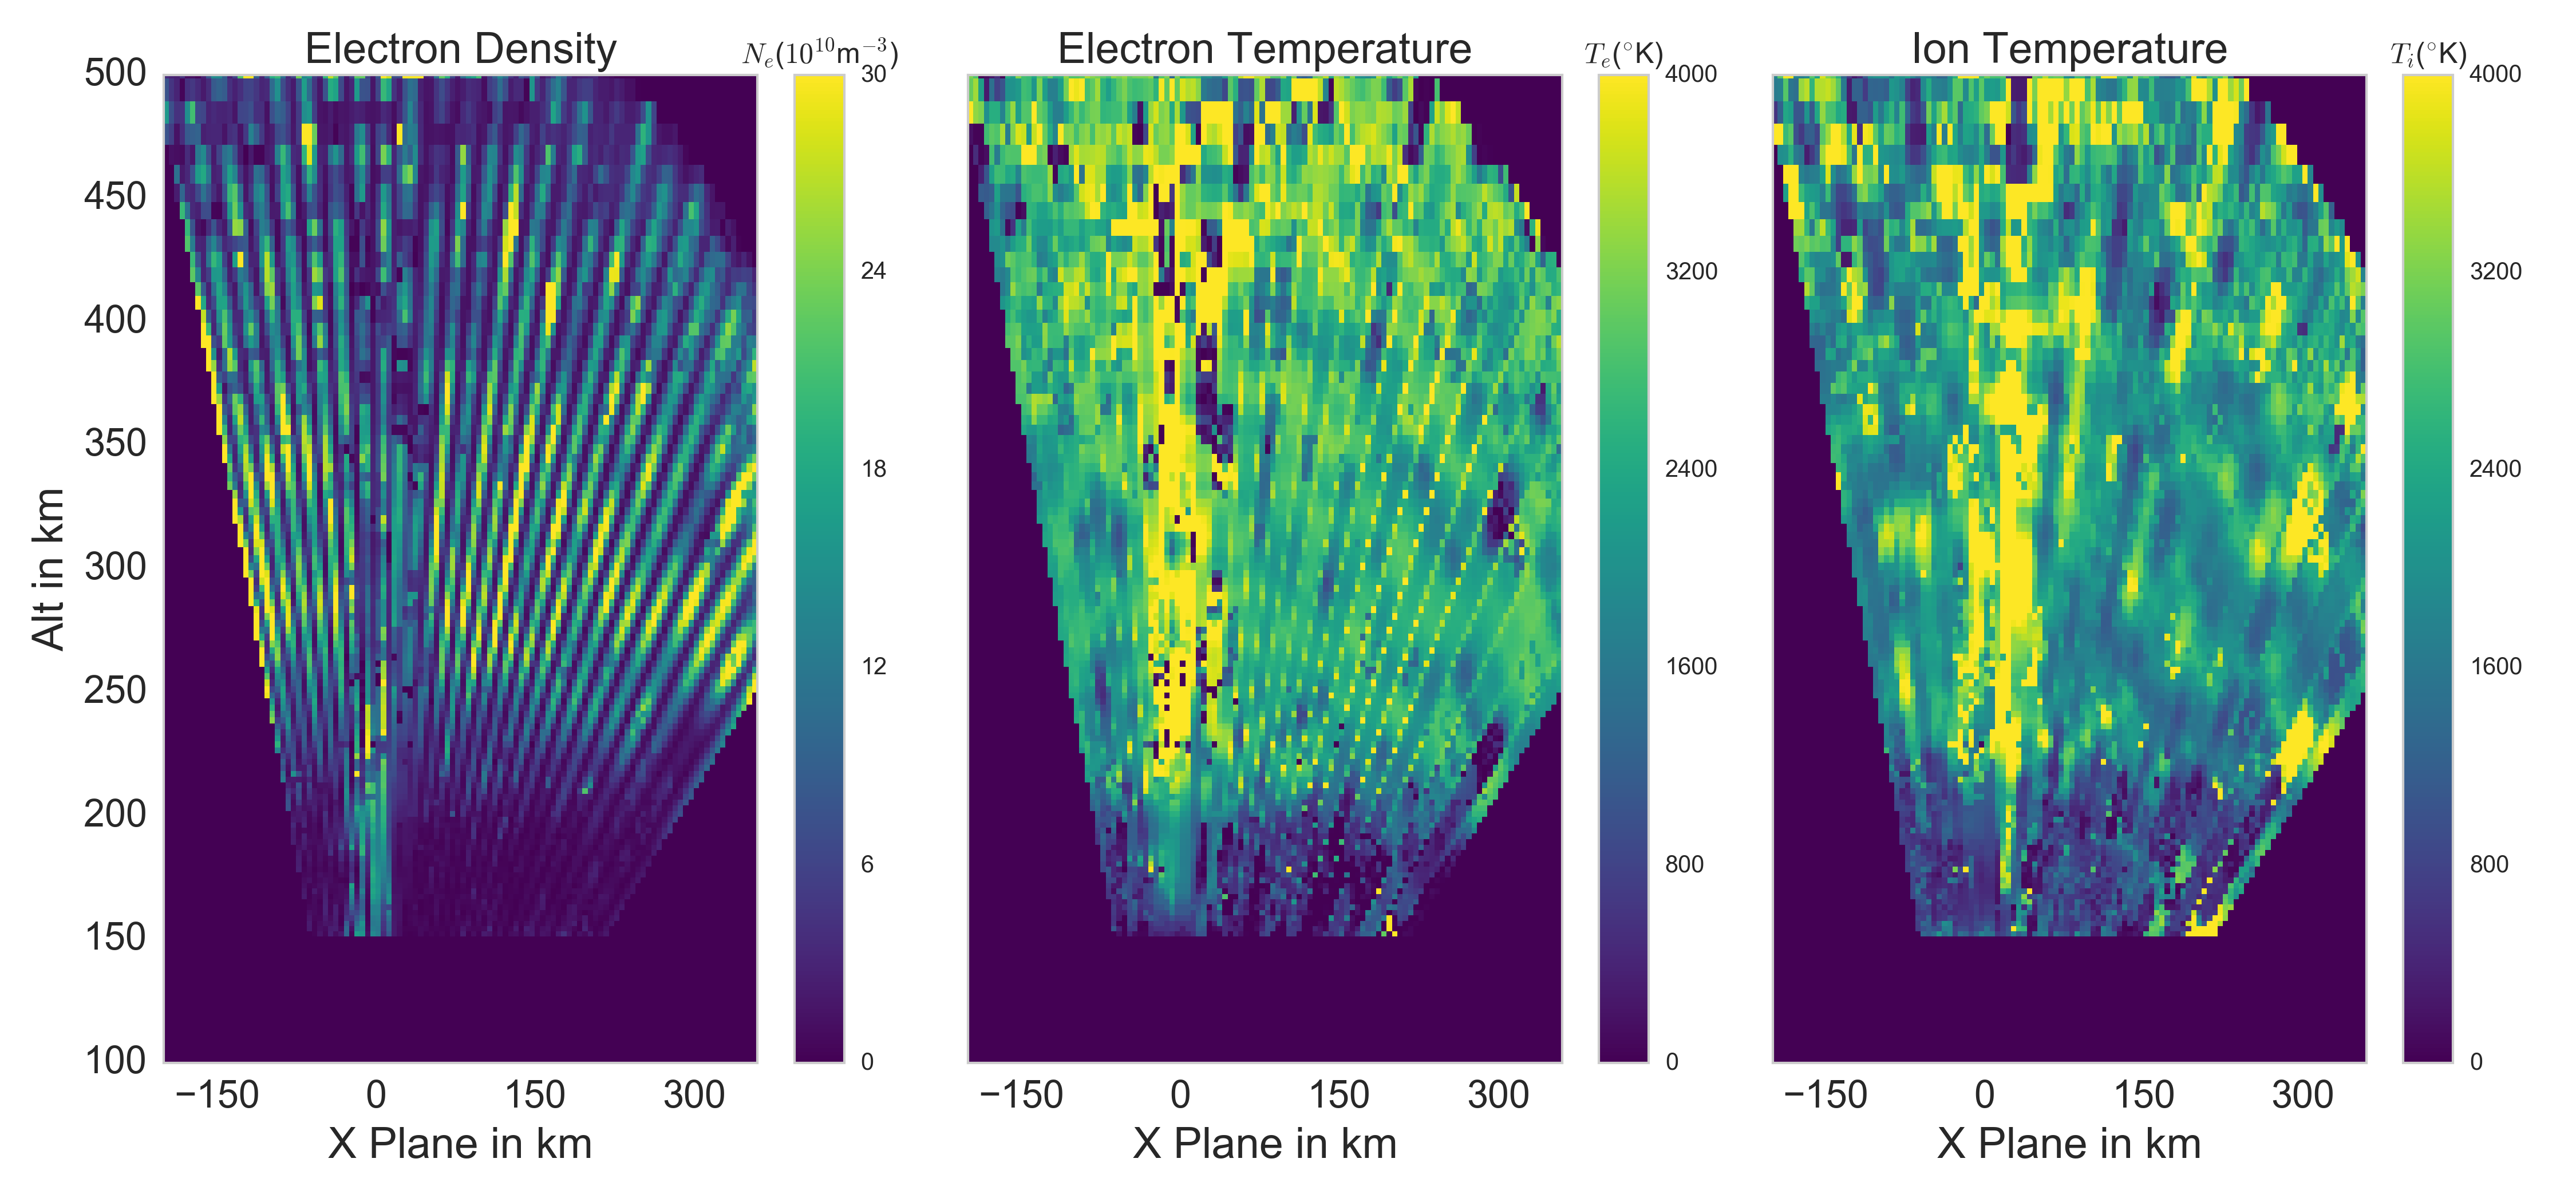
\includegraphics[width=6in]{tikfitted}
\caption{Fitted Plasma Parameters at $t=960$ s inverting lags with Equation \ref{eqn:tikpow}}
\label{fig:tikpow}
\end{figure}

The image in Figure \ref{fig:tikD} is the result of using Tikhonov regularization on the spatial gradient of each lag of the ACF. This leads to an apparent smoothing of the plasma parameter but many of the important features in this simulation, such as the depletion in $N_e$ and enhancements in $T_e$ and $T_i$ are visible and more obvious than in Figure \ref{fig:fplparamst60}
\begin{figure}[!ht]
\centering
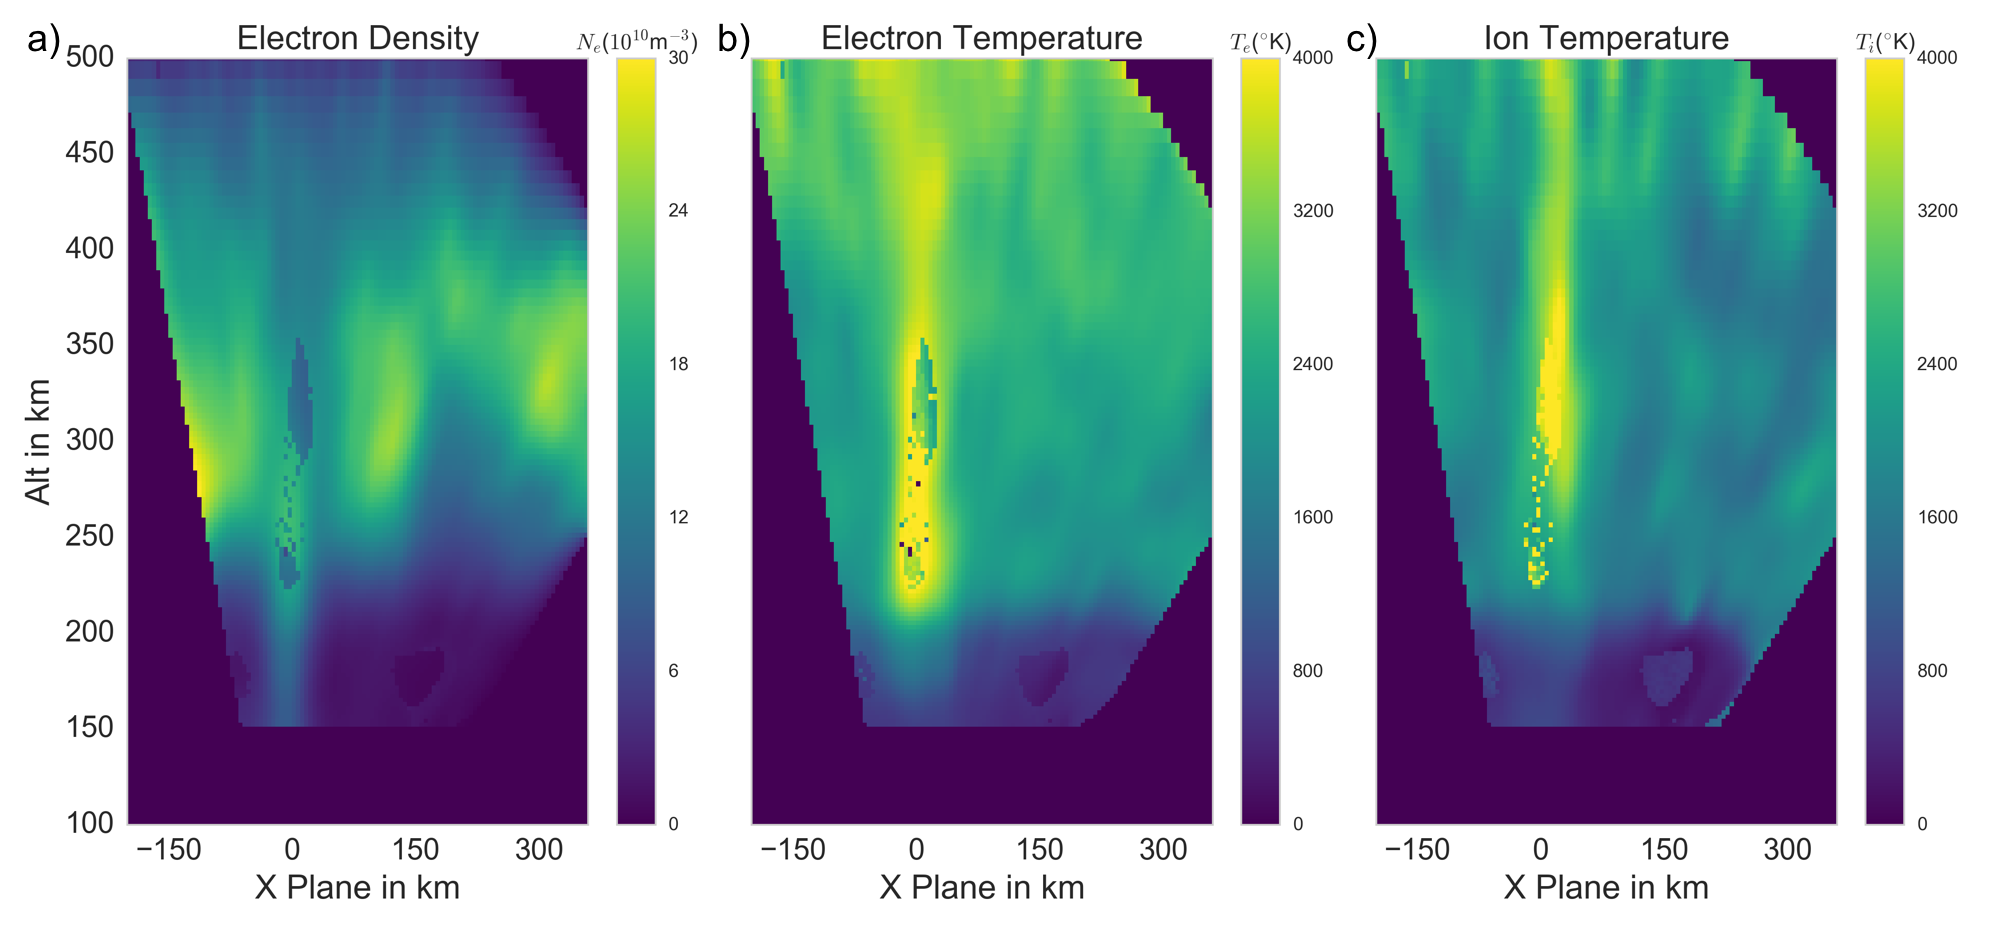
\includegraphics[width=6in]{tikdfitted}
\caption{Fitted Plasma Parameters at $t=960$ s inverting lags with Equation \ref{eqn:tikD}}
\label{fig:tikD}
\end{figure}

Lastly for this case the result of the inversion using the total variations constraint is shown in Figure \ref{fig:tv}. This inversion method does the features discussed earlier but they take on a "blocky" look. This can be expected for total variations as has been very popular in use of reconstructing high contrast images\cite{Karl:2005jy}.
\begin{figure}[!ht]
\centering
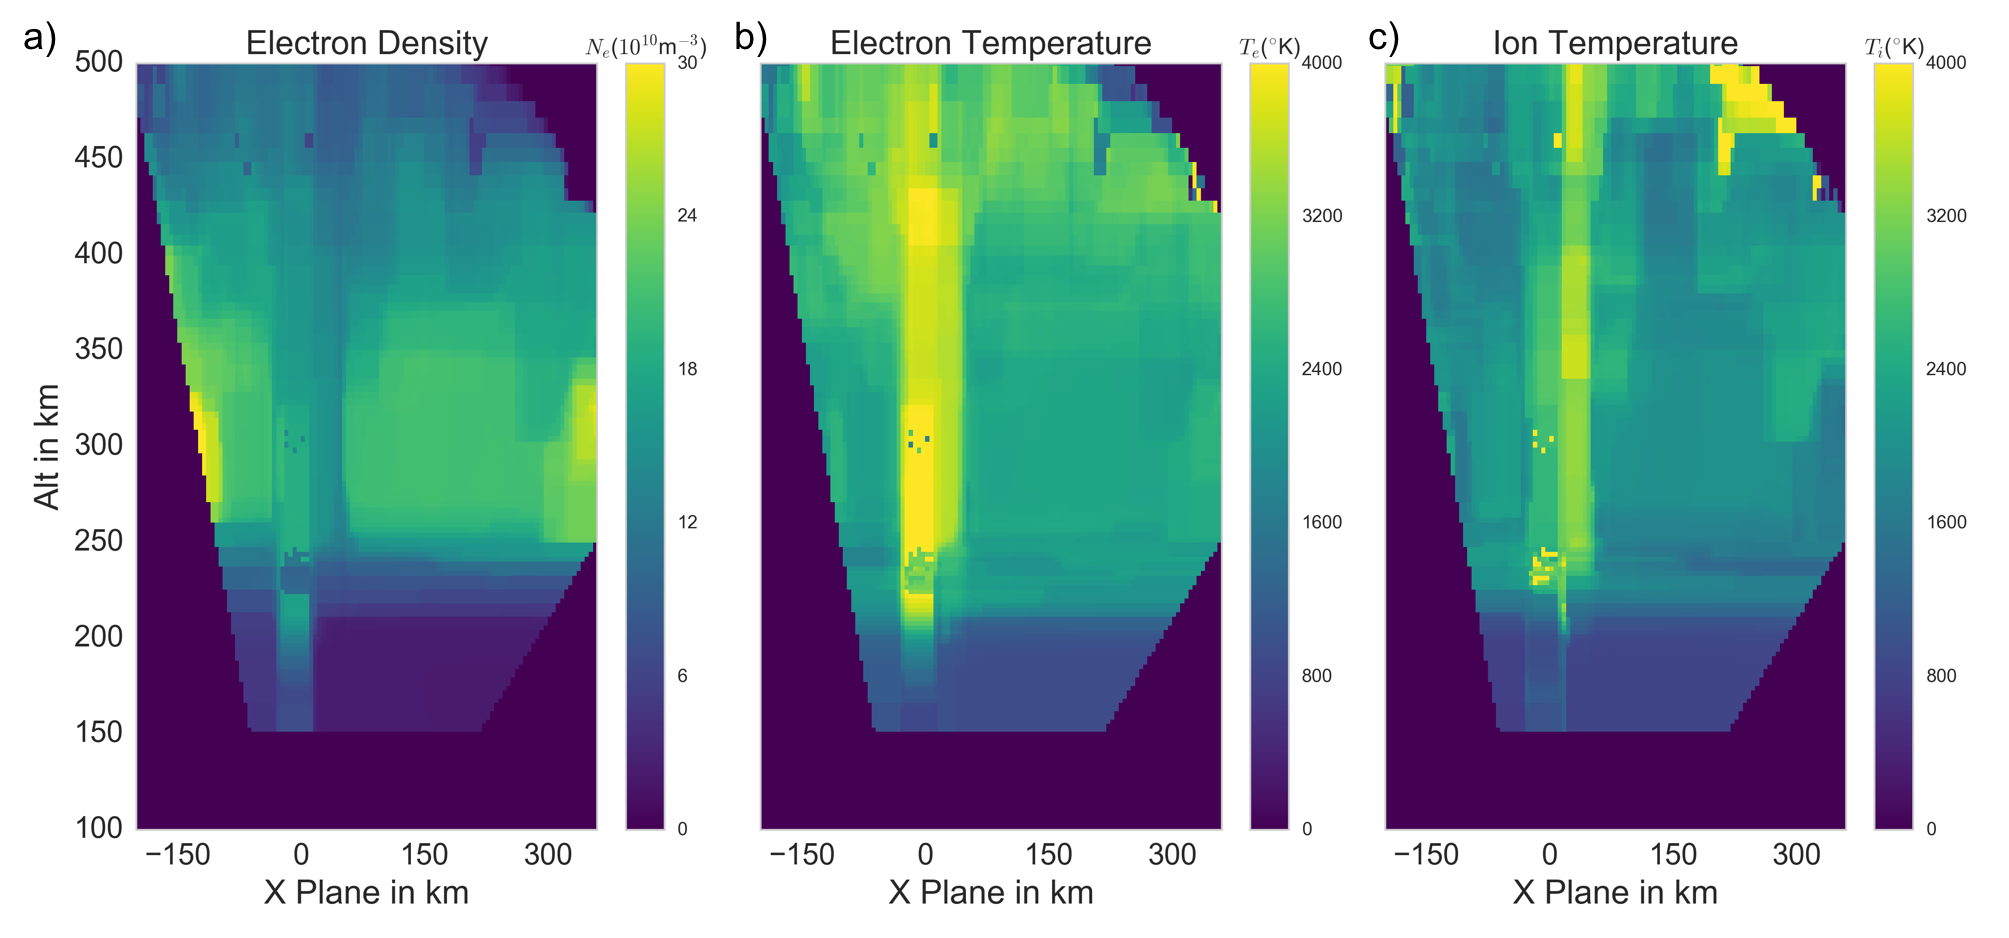
\includegraphics[width=6in]{tvfitted}
\caption{Fitted Plasma Parameters at $t=960$ s inverting lags with Equation \ref{eqn:tv}}
\label{fig:tv}
\end{figure}

\section{Conclusions}

This article has discussed the different ways to reconstruct plasma parameters from ESA ISR. A basic overview of different reconstruction schemes currently in the literature was shown. Following that the different reconstruction schemes from single beam ISR systems was covered and were broken down into parametric vs data based regularization. We then discuss our own reconstruction scheme using a regularization scheme on the lag data. We show reconstructions from the technique from a multi-fluid model simulation of the ionosphere.
